\subsection{Network Analysis}\label{sec_res_nets}
        
        Section \ref{sec_res_exp} presented support for the hypothesis that right-leaning Twitter users hold strong anti-immigration views and are more active on Twitter. In order to analyze whether this higher activity level also translates to more influence in online conversations, we use network analysis methods to provide descriptive evidence on the most active users, the most influential users and the interconnectedness within left- and right-leaning Twitter users. (We provide a brief mathematical walkthrough of the measures utilized in this section in Appendix \ref{appsec_theory_net}. Practitioners can skip this appendix.)  
        
        
    \paragraph{General Network Description}
       
        Our general retweet network is described by the graph $G=(E,V)$, where $V$ is the set of vertices consisting of the 45,525 Chilean Twitter users, and $E$ is the set of edges consisting of the 578,383 retweets among users. The edges are directed from the person retweeting  to the person being retweeted. The links are weighted by total number of times a person $A$ retweeted a person $B$. For our particular case, the weights are ranging from 1 (representing a unique retweet) to the maximum of 532. We use retweets as links following the literature and the previous practices of the Chilean Communication Office.
        
        Figure \ref{fig_entire_graph_1000} presents a simplified visualization of the retweet network between users. We find two clusters: one of right-leaning users and one of left-leaning users. Right-leaning users seem more prominent and more densely connected, while left-leaning users are more spread out. Considering the recent runner-up in the presidential election, the right-leaning politician José Kast, we find that he is more central in his right-wing cluster while the current left-wing president Gabriel Boric is less central in his left-wing cluster. Unlabeled users are more densely connected to the right-leaning users, however some of them are connected to left-leaning users to a higher degree. We investigate this further in Section \ref{unlab_users_affiliation}.


%Figure \ref{fig_net_entire_graph} presents a visualization of the network with the 150 most influential users. In the figure, mostly right-leaning users are visible (red dots), there are a few unlabeled ones (yellow dots) and even fewer left-leaning nodes (blue dots). We find that the right-wing candidate José Kast is quite central in the cluster of right-leaning users, while left-wing president Gabriel Boric is distanced from the left-leaning Twitter users. 

        
        \begin{figure}[H]
             \centering
             %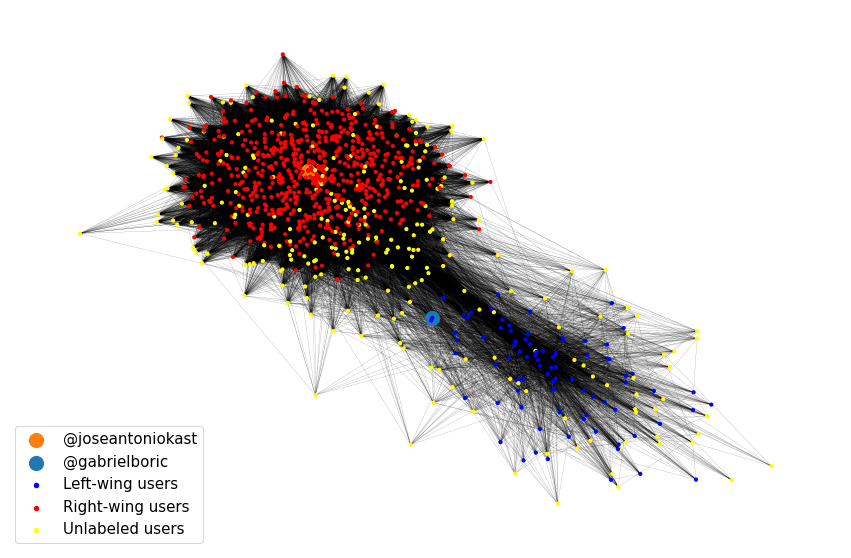
\includegraphics[width=.85\textwidth]{figs/thesis_entire_graph_1000.png}
             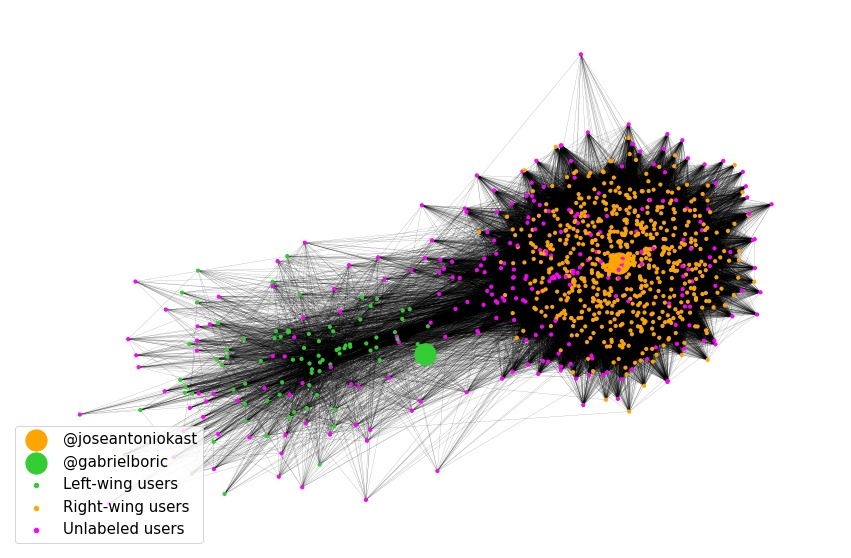
\includegraphics[width=.85\textwidth]{figs/thesis_entire_graph_1000_2.jpeg}
             \caption{Simplified Undirected General Graph of Retweet Network}
             \label{fig_entire_graph_1000}
             
             \floatfoot{\it 
                    Notes:  The network plot is undirected and considers the 1,000 most important users in terms of degree centrality.\\ 
                    Data Source: Retweets network retrieved from Twitter API and \texttt{twarc2}'s network plug-in. Result of Step 8 of the applied methodology as described in Section \ref{sec_meth_gene} and Appendix \ref{app_sec_meth}.}
        \end{figure}

  
            \newline\noindent  
         In order to measure the retweet activity of Twitter users across political affiliation, we consider differences of degree measures. Since the graph is directed, we can differentiate between the volume of retweets received (terminologically called ''in-degree'') and sent (terminologically called ''out-degree''). From Table \ref{tab_net_measure_volume} we find that among the 1,000 Twitter users with the highest degree measures, right-leaning and unlabeled users get significantly more tweets retweeted. This is in line with the findings of higher activity from right-leaning users from Table \ref{tab_corp_charac_subs} in Section \ref{sec_res_exp}. For those users that retweet others, the contrast is even starker. Here right-leaning users retweet significantly more than both left-leaning as well as unlabeled users. Given this information, we find that right-leaning users are the most active about immigration, but might not have the greater influence given the important presence of unlabeled nodes.


        \begin{table}[!htb]
                %\footnotesize
                \centering
                
                \subfile{tabs/net_measure_volume}
                
                %\caption{Degree Measures (retweet volume) for Top 1,000 Twitter Users}
                \caption{Degree Measures for Top 1,000 Twitter Users}
                
                \floatfoot{\it 
                %Notes:  \\ 
                Data Source: Retweets network retrieved from Twitter API and \texttt{twarc2}'s network plug-in. Result of Step 8 of the applied methodology as described in Section \ref{sec_meth_gene} and Appendix \ref{app_sec_meth}.}
                
                \label{tab_net_measure_volume}
            \end{table}
        
        %Given that right-wing users are most active in retweets, yields the suspicion that some of these accounts might be bots or fake accounts. In fact, as an example we find the user \texttt{@j-pablo-escobar} with an out-degree measure of 639 which is an account that has no picture, only a fake and famous alias. The bio states {\it "Patriota, Republicano, voto por kast"} (Eng: "Patriot, Republican, vote for Kast"). Upon manual inspection of this user's activity, we find that the retweets consist of controversial facts, or opinion polls which enables his right-leaning followers to spread these views. Hence, it seems there are some fake accounts in our corpus as is further discussed in Section \ref{sec_disc_improv}.


    \paragraph{Influence}

        We have found that right-leaning users %and unlabeled ones 
        are the most active ones. In order to measure whether this higher activity translates into influence, we identify the most influential users using two different centrality measures: Degree centrality and eigenvector centrality. Degree centrality measures the influence of users based on their retweets, while eigenvector centrality measures the influence, based on the influence of their nearest neighbors. Table \ref{tab_net_meas} presents the 1,000 most influential Twitter users. Using both measures, the general pattern is the same. We find that more than 60\% of the most influential users are right-leaning. The influence of left-leaning and unlabeled users slightly depends on the centrality measure, but generally unlabeled users are more influential than left-leaning users. Hence, the general pattern throughout our findings also holds in terms of influence: Right-leaning Twitter users are more influential than left-leaning ones on the topic of immigration.


        \begin{table}[!htb]
                %\footnotesize
                \centering
                
                \subfile{tabs/net_measure_cent}
                
                %\caption{Centrality Measures (retweet influence) for Top 1,000 Twitter Users}
                \caption{Centrality Measures for Top 1,000 Twitter Users}
                
                \floatfoot{\it 
                %Notes:  \\ 
                Data Source: Retweets network retrieved from Twitter API and \texttt{twarc2}'s network plug-in. Result of Step 8 of the applied methodology as described in Section \ref{sec_meth_gene} and Appendix \ref{app_sec_meth}.}
                
                \label{tab_net_meas}
            \end{table}
    
        To identify the most influential users, Table \ref{tab_net_degree_cent} presents the five Twitter users from our corpus with the highest degree centrality measure (by eigenvector centrality in Appendix Table \ref{apptab_net_5_eigenvector}). The account of the right-leaning politician José Kast (runner-up in the recent presidential election) is the most influential Twitter user. This could be explained from the findings from Figure \ref{fig_hashtags_protest_rig} in Section \ref{sec_res_exp} that Kast's supporters used endorsing hashtags during the September 2021-protests such as \texttt{\#atraveteconkast} (Eng: Go with Kast) and \texttt{\#kastpresidente} (Eng: President Kast).
        
        The unlabeled nodes found in the most influential users are mainly celebrities (\texttt{@AldoDuqueSantos}) and media outlets: television program \texttt{@T13} and radios \texttt{@Biobio} and \texttt{@Cooperativa}. The current president and left-wing leader is only found in 146\textsuperscript{th} place as measured by degree centrality (7\textsuperscript{th} among left-leaning users, see Appendix Table \ref{apptab_net_degree_polaff}) and 799\textsuperscript{th} by eigenvector centrality (3\textsuperscript{rd} among left-leaning users, see Appendix Table \ref{apptab_net_eigen_polaff}). Hence the President is influential within left-leaning users but (given their general low influence level) not influential in the general Chilean Twittersphere.
        
        
        Generally, we find right-leaning users to be more active than the left-leaning ones in the topic of immigration. However, in terms of influence, many unlabeled users have high scores, not solely right-leaning users.


        \begin{table}[!htb]
            %\footnotesize
            \centering
            
            \subfile{tabs/net_10_influential}
            
            \caption{Five Most Influential Users by Degree Centrality}
            
            \floatfoot{\it 
            %Notes:  \\ 
           Data Source: Retweets network retrieved from Twitter API and \texttt{twarc2}'s network plug-in. Result of Step 8 of the applied methodology as described in Section \ref{sec_meth_gene} and Appendix \ref{app_sec_meth}.}
            
            \label{tab_net_degree_cent}
        \end{table}


%        \begin{figure}[H]
%             \centering
             %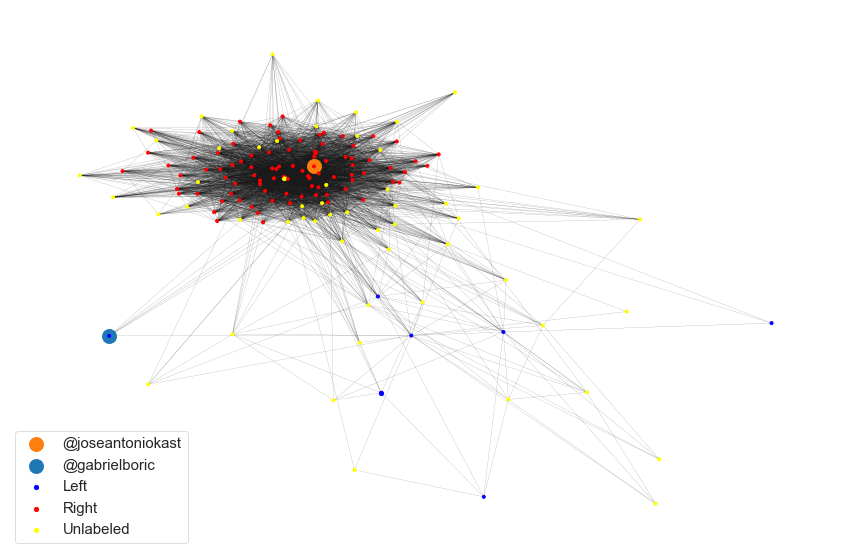
\includegraphics[width=.80\textwidth]{figs/thesis_entire_graph.png}
             %\caption{Top 150 Influential Users in the Network}
             %\label{fig_net_entire_graph}
             %\floatfoot{\it 
                    %Notes: Influence measured by degree centrality. \\ 
                    %Data Source: \textcolor{red}{$<$mention the corpus where this comes from á la footnote in Table \ref{tab_corpora_characs}$>$}}
        %\end{figure}

        %Figure \ref{fig_net_entire_graph} presents a visualization of the network with the 150 most influential users. In the figure, mostly right-leaning users are visible (red dots), there are a few unlabeled ones (yellow dots) and even fewer left-leaning nodes (blue dots). We find that the right-wing candidate José Kast is quite central in the cluster of right-leaning users, while left-wing president Gabriel Boric is distanced from the left-leaning Twitter users. 
    
    
    
    \paragraph{Interconnectedness}
    
        In order to analyze the interconnectedness of Chilean Twitter users across political affiliations, we consider the two metrics of density and reciprocity. The measures are conceptually similar. Reciprocity measures the probability that two authors in the network retweet each other. Density measures the proportion of retweets among all possible pairs of users in the network. To measure political affiliation-specific interconnectedness, we built two separate subnetworks: One only containing right-leaning Twitter users, the other only containing left-leaning users. Table \ref{net_dens_rec} shows that right-leaning Twitter users retweet each other more than the left-leaning Twitter users do, and hence are more interconnected. Right-leaning users are also more interconnected than the aggregate network. 
        
        
        \begin{table}[!htb]
                %\footnotesize
                \centering
                
                \subfile{tabs/net_dens_rec}
                
                \caption{Interconnectedness Measures}
                
                \floatfoot{\it 
                %Notes:  \\ 
                Data Source: Retweets network retrieved from Twitter API and \texttt{twarc2}'s network plug-in. Result of Step 8 of the applied methodology as described in Section \ref{sec_meth_gene} and Appendix \ref{app_sec_meth}.}
                
                \label{net_dens_rec}
            \end{table}
        
        
            \newline\indent
        Generally, we find that right-leaning users are more active and well-connected than left-leaning users. Our results also indicate that unlabeled users to a large extent are right-leaning, but not to a all-encompassing extent.
        
        
    %\subsection{Misclassified User Accounts}    
        
    %\paragraph{Unlabeled Users}\label{unlab_users_affiliation}
        
    %    To further analyze the characteristics of the unlabeled users we can compare the findings from the networks metrics with those from the textual results. 

     %       \newline\indent
     %   Figure \ref{fig_bigram_protest_unlab} gives insights as to which ideology is most prevalent in the 'Unlabeled' category. The distribution of bigrams is more akin to that of the right-leaning users and so are the connotations of the bigrams. We find unlabeled users to mainly stress the undocumented/illegal situation of the migrants with popular bigrams such as {\it 'inmigrantes, ilegales'} (Eng: Immigrants, illegals), {\it 'crisis, migratoria'} (Eng: Crisis, migratory), {\it 'marcha, encontra'} (Eng: March, against) and {\it 'encontra, migrantes'} (Eng: Against, migrants). So in the unlabeled category we find that these are more similar to right-leaning users. Either we have some right-leaning users in the 'Unlabeled' category that our labeling strategy classifies wrongly. It could also be the case that unlabeled users are in fact center-leaning and that center voters are more anti-immigration than embracing. This supports the finding from Figure \ref{fig_entire_graph_1000} that unlabeled users are mostly centered close to right-leaning users.
    
     %       \newline\indent
        %However, one finding points towards that the 'Unlabeled' category mainly includes right-leaning individuals. There are some common bigrams for unlabeled users that neither left-leaning nor right-leaning users use. This is specifically the mention of the UN ({\it 'ONU'} in Spanish). In Figure \ref{fig_bigram_protest_unlab} the mention of \texttt{@onuchile} is prevalent, while Figure \ref{fig_hashtags_protest_unlab} shows that hashtags such as \texttt{\#fueraonu} (Eng: Out with the UN) and \texttt{\#nomasonu} (Eng: No more UN) are popular among unlabeled users. This shows that these users argue that the UN is to blame for the uncontrolled immigration. 
      %  We also find frequent usage of hashtags such as \texttt{\#nomasinmigrantes} (Eng: No more immgirants) and \texttt{\#nomasinmigrantesilegales} (Eng: No more illegal immigrants) which mainly mirror the talking points of the right. However, we find one specific talking point from the left-leaning users which is \texttt{\#xenofobia} (Eng: Xenophobia). With these findings in mind, we cannot claim that unlabeled users primarily are right-leaning as the use of hashtags is ambiguous across ideological agendas. This is again consistent with findings from Figure \ref{fig_entire_graph_1000} that unlabeled users seem most similar to right-leaning users, but that there is a minority more similar to left-leaning users.
        
      %      \newline\indent
      %  Generally, it seems that unlabeled users are primarily reminiscent of the right-leaning users. 
        %and if we assume anti-UN sentiments to be right-wing agendas, it could be a reasonable assumption that unlabeled users are primarily right-leaning. In this case, the previous findings, e.g. those from Figure \ref{fig_terms}, could potentially be even starker. 
     %   More accurately categorizing the unlabeled users is therefore one of the most immediate future improvements to our project as is further discussed in Section \ref{sec_disc_improv}.
        
    
    %\paragraph{Fake Accounts}
    %    The results from Table \ref{tab_net_measure_volume} showed that right-wing users are most active in retweets. This raised the suspicion that some of these accounts might be bots or fake accounts. In fact, as an example we find the user \texttt{@j-pablo-escobar} with an out-degree measure of 639 (meaning this user sends a high number of retweets). This is an account that has no picture, only a fake and famous alias. The bio states {\it "Patriota, Republicano, voto por kast"} (Eng: "Patriot, Republican, vote for Kast"). Upon manual inspection of this user's activity, we find that the retweets consist of controversial facts, or opinion polls which enables his right-leaning followers to spread these views. Hence, it seems there are some fake accounts in our corpus as is further discussed in Section \ref{sec_disc_improv}.